\section{Definisi Data Spasial (GEOGRAPHICS INFORMATION SYSTEM)}
Data Spasial Sistem Informasi Geografis (SIG) model data yang akan digunakan dari bentuk dunia nyata harus dapat diimplementasikan ke dalam basisdata. Data ini dimasukkan ke dalam komputer yang nantinya memanipulasi objek dasar yang memiliki atribut geometri (entity spasial/entity geografis) 
(Prahasta, 2002a). Data spasial pada dasarnya dapat disimpulkan bahwa data spasial merupakan suatu entitas data dalam Sistem Informasi Geografis (SIG) yang dapat dikelola, dianalisa dan dapat memetakan informasi objek keruangan beserta data-data atributnya serta dapat disimpan di dalam database yang dapat ditampilkan kedalam suatu sistem tertentu sehingga dapat mendukung dalam pengambilan keputusan. 

\subsection{Model data Vektor pada Geographics Information System GIS}
Vektor  pada GIS mampu melakukan penempatan, menampilkan data spasial bahkan menyimpan datanya yang menggunakan titik-titik, garis-garis dan juga poligon yang dilengkapi dengan artibut-artibutnya. Bentuk-bentuk dasar representasi dari data spasial ini di dalam sistem model data vektor dapat didefinisikan oleh sistem koordinat kartesian dua dimensi (X,Y). Dimana di dalam model data spasial vektor, garis-garis atau kurva (busur atau arcs) adalah berupa sekumpulan titik-titik terurut yang saling berhubungan (Prahasta, 2002a). 

\subsubsection{Model data Vektor dengan bentuk point/titik pada Geographics Information System GIS}
Point/titik merupakan representasi grafis yang paling sederhana pada suatu objek. titik pada data vektor tidak mempunyai dimensi tetapi bisa ditampilkan ke dalam bentuk simbol baik pada peta maupun dalam layar monitor. contoh  lokasi fasilitas kesehatan, kantor pemerintah dan lain-lain.
Pada gambar \ref{point} dijelaskan bahwa gambar point/titik data vektor GIS sebagai berikut.
\begin{figure}[ht]
	\centerline{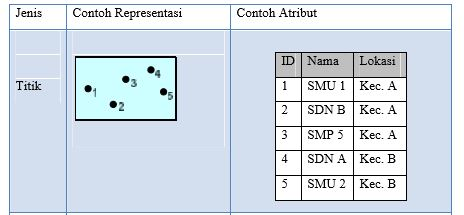
\includegraphics[width=1\textwidth]{figures/point.JPG}}
	\caption{point.}
	\label{point}
	\end{figure}

Maka artikel :
	Dalam sebuah artikel dari husein yang menyebutkan bahwa  GIS merupakan pemahaman dari
	Geography, Information dan System \cite{widiatmoko2009aplikasi}.

\subsection{Contoh Proses Data Geospatial}
data disimpan Misalnya dalam spesies berikut kejadian analisis akan yang digunakan untuk menggambarkan geospasial pengolahan data dalam sistem kepler.Tujuannya adalah untuk menemukan berbagai spesies baris ini dari a yang di dalam persimpangan dari lambung cembung baris ini dari spesies b dan spesies c.Kejadian datasets kami beranggapan bahwa al ( point data ) disimpan dalam tiga format-format antara lain :
